
\begin{center}
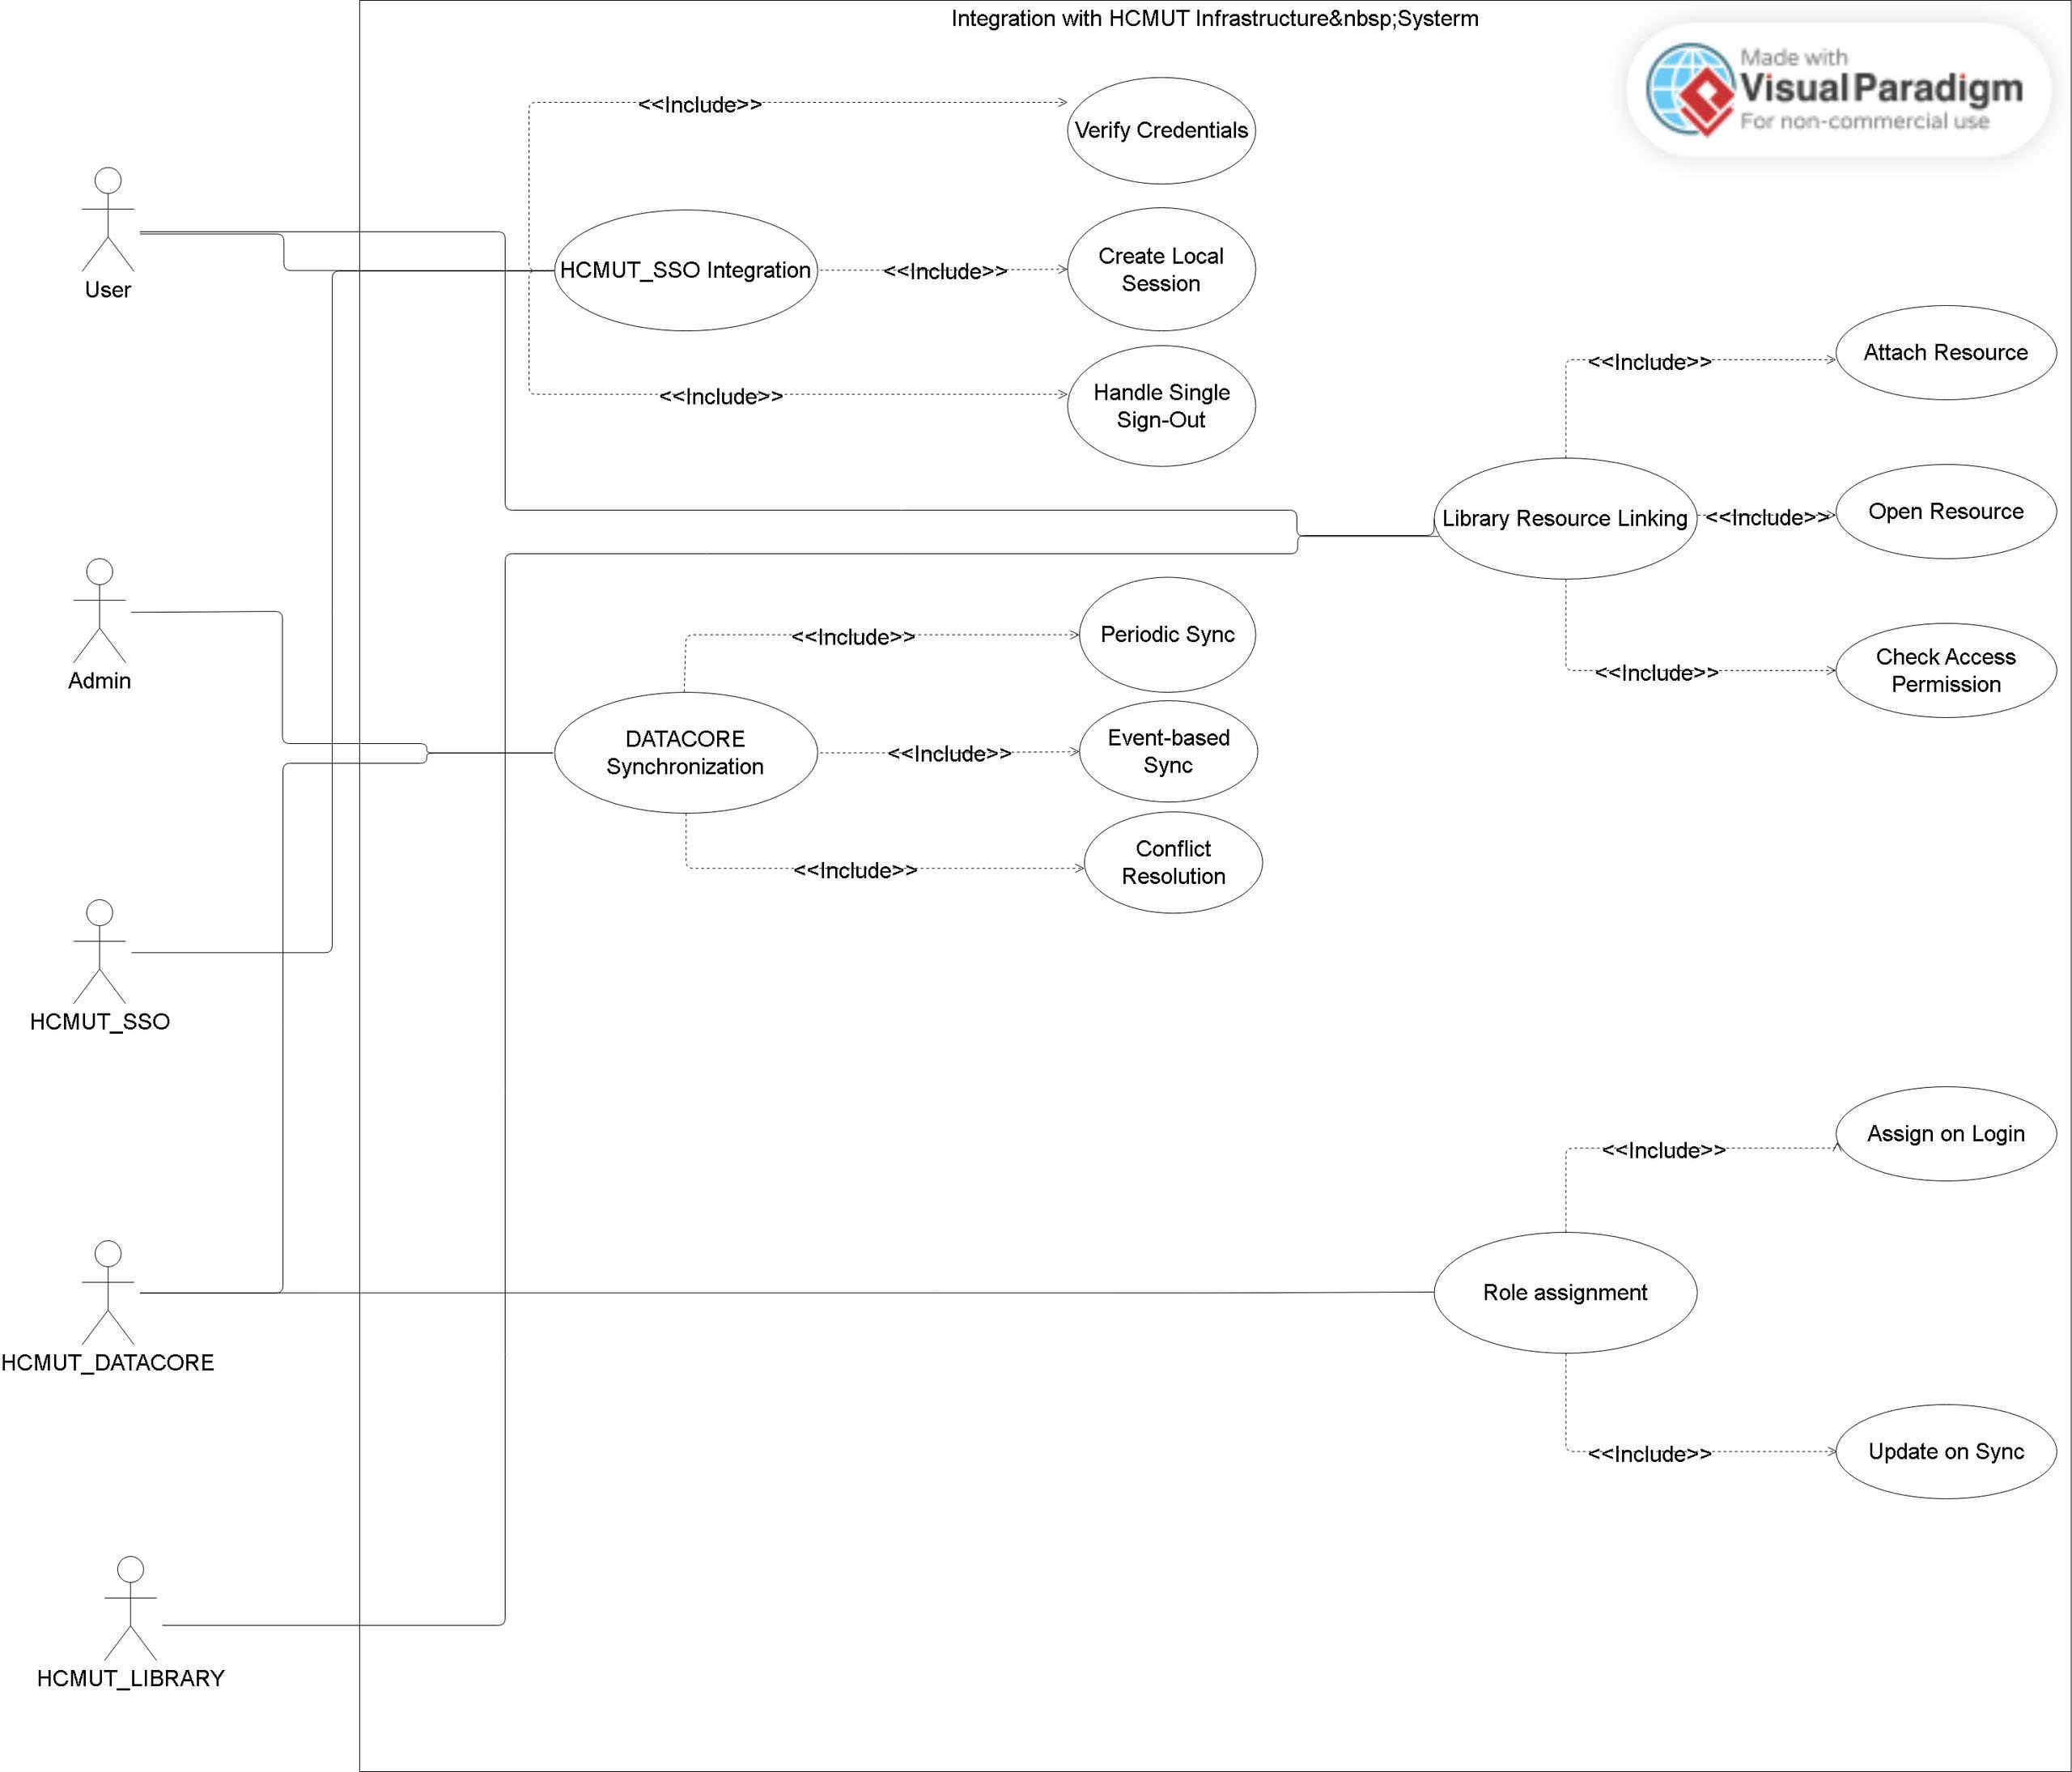
\includegraphics[width=0.9\linewidth]{images/UC-06.png}
\end{center}

\begin{center}
\textbf{Figure 7:}  Integration with HCMUT Infrastructure
\end{center}

\begin{table}[h!]
\centering
\begin{tabular}{|p{3cm}|p{11cm}|}
\hline
\textbf{Use-case ID} & UC-06.01 \\
\hline
\textbf{Use-case name} & HCMUT\_SSO Integration \\
\hline
\textbf{Use-case overview} & The system integrates with HCMUT\_SSO for unified authentication, allowing users to log in using university credentials and automatically manage single sign-out. \\
\hline
\textbf{Actors} & User, System, HCMUT\_SSO \\
\hline
\textbf{Preconditions} & HCMUT\_SSO service is operational and reachable. \\
\hline
\textbf{Trigger} & User initiates login via HCMUT\_SSO. \\
\hline
\textbf{Steps} & 
1. User selects “Login with HCMUT\_SSO”. \newline
2. System redirects to the authentication portal. \newline
3. HCMUT\_SSO validates credentials and returns a token. \newline
4. System verifies the token and creates a session. \newline
5. Upon sign-out at SSO, the system terminates the local session. \\
\hline
\textbf{Postconditions} & 
1. User is successfully authenticated. \newline
2. Single sign-out ensures session consistency. \\
\hline
\textbf{Exception Flow} & 
1. Invalid or expired token → login attempt rejected. \newline
2. SSO service unavailable → system displays maintenance message. \\
\hline
\textbf{Priority} & Must \\
\hline
\end{tabular}
\caption{Use Case UC-06.01: HCMUT\_SSO Integration}
\end{table}


\begin{table}[h!]
\centering
\begin{tabular}{|p{3cm}|p{11cm}|}
\hline
\textbf{Use-case ID} & UC-06.02 \\
\hline
\textbf{Use-case name} & DATACORE Synchronization \\
\hline
\textbf{Use-case overview} & The system synchronizes personal and academic data from HCMUT\_DATACORE periodically or in near real-time to ensure data consistency and reduce manual entry. \\
\hline
\textbf{Actors} & System, HCMUT\_DATACORE, Administrator \\
\hline
\textbf{Preconditions} & DATACORE APIs are online and accessible. \\
\hline
\textbf{Trigger} & Scheduled synchronization or data-change event detected. \\
\hline
\textbf{Steps} & 
1. System triggers synchronization with DATACORE. \newline
2. Retrieve updated profiles and academic data. \newline
3. Validate and compare data with local records. \newline
4. Update local data using DATACORE as source of truth. \newline
5. Log synchronization status and timestamp. \\
\hline
\textbf{Postconditions} & 
1. Local data mirrors DATACORE. \newline
2. Synchronization events logged for auditing. \\
\hline
\textbf{Exception Flow} & 
1. Connection timeout or API error → retry with exponential backoff. \newline
2. Invalid data format → skip record and log validation error. \\
\hline
\textbf{Priority} & Must \\
\hline
\end{tabular}
\caption{Use Case UC-06.02: DATACORE Synchronization}
\end{table}

\begin{table}[h!]
\centering
\begin{tabular}{|p{3cm}|p{11cm}|}
\hline
\textbf{Use-case ID} & UC-06.03 \\
\hline
\textbf{Use-case name} & Role Assignment \\
\hline
\textbf{Use-case overview} & The system automatically assigns user roles (student, tutor, coordinator, department chair, or administrator) based on centralized role data from DATACORE and SSO. \\
\hline
\textbf{Actors} & User, System, HCMUT\_DATACORE \\
\hline
\textbf{Preconditions} & User is authenticated via SSO and DATACORE role data is available. \\
\hline
\textbf{Trigger} & User login or scheduled role update. \\
\hline
\textbf{Steps} & 
1. Retrieve role mapping from DATACORE. \newline
2. Match user ID with centralized role data. \newline
3. Assign permissions based on role. \newline
4. Apply changes in access-control policies. \newline
5. Log the role-assignment event. \\
\hline
\textbf{Postconditions} & 
1. User roles align with centralized data. \newline
2. Updated permissions take effect immediately. \\
\hline
\textbf{Exception Flow} & 
1. Role data missing → assign default “student” role and notify admin. \newline
2. Role conflict → logged and flagged for manual verification. \\
\hline
\textbf{Priority} & Must \\
\hline
\end{tabular}
\caption{Use Case UC-06.03: Role Assignment}
\end{table}


\begin{table}[h!]
\centering
\begin{tabular}{|p{3cm}|p{11cm}|}
\hline
\textbf{Use-case ID} & UC-06.04 \\
\hline
\textbf{Use-case name} & Library Resource Linking \\
\hline
\textbf{Use-case overview} & The system connects with HCMUT\_LIBRARY to let tutors and students attach or access library materials securely within tutoring sessions or summaries. \\
\hline
\textbf{Actors} & Student, Tutor, System, HCMUT\_LIBRARY \\
\hline
\textbf{Preconditions} & Library API and authentication services are available. \\
\hline
\textbf{Trigger} & User attaches or opens a library resource. \\
\hline
\textbf{Steps} & 
1. User searches or selects a library resource. \newline
2. System requests metadata and access permissions. \newline
3. Verify user eligibility via role-based access. \newline
4. Attach or open the resource in session view. \newline
5. Log the access event. \\
\hline
\textbf{Postconditions} & 
1. Resource successfully linked to the session or summary. \newline
2. Access rights enforced per library policy. \\
\hline
\textbf{Exception Flow} & 
1. Access denied → system displays permission error. \newline
2. Library service unavailable → prompt user to retry or queue attachment. \\
\hline
\textbf{Priority} & Could \\
\hline
\end{tabular}
\caption{Use Case UC-06.04: Library Resource Linking}
\end{table}

